\documentclass[a4paper, 10pt]{article}
\usepackage{scrextend}
\changefontsizes{9pt}
% Per-subject config for this repo. See vendor/template/course-config.tex.example
% for what each macro is used for.

\newcommand{\CourseCode}{2110413}
\newcommand{\CourseName}{Computer Security}
\newcommand{\StudentID}{6733172621}
\newcommand{\StudentName}{Patthadon Phengpinij}
\newcommand{\DefaultCollaborators}{Claude (for\,\LaTeX\,styling and grammar checking)}
\newcommand{\AssignmentLabel}{Activity}

\usepackage{../vendor/template/CEDT-Assignment-style}
\usepackage[normalem]{ulem}
\usepackage{newunicodechar}
% Inconsolata has no U+FFFD (replacement character), so borrow that one glyph from FreeMono.
\newfontfamily\replacementcharfont{FreeMono}[Scale=MatchLowercase]
\newunicodechar{�}{{\replacementcharfont\char"FFFD\relax}}

\begin{document}
\subject
\asgntitle{4}{}{Fundamentals of Cryptography}{\StudentID\ \StudentName}{\DefaultCollaborators}

% ================================================================================ %
\section*{Overviews}
% ================================================================================ %

\par \myspace[h] In this activity, we will learn the basics of encryption.
There are 3 exercises in this activity.
Each exercise is designed to let you learn the concepts of cryptography.
We will need:
\begin{itemize}
	\item \texttt{ImageMagick}
	\item \texttt{OpenSSL}
	\item One of your favorite programming languages.
\end{itemize}
You are welcome to do this exercise with any programming language.
If you have no preference, use \texttt{Python}.

% ================================================================================ %
\section*{Exercises}
% ================================================================================ %

% ================================================================================ %
%                                    Problem 01                                    %
% ================================================================================ %
% TODO: replace with the time you actually measured when cracking the text by hand.
\newcommand{\ManualCrackTime}{15 minutes}

\begin{problem}
\textbf{(Cryptanalysis)}
\par Though encryption is primarily designed to preserve confidentiality and integrity of data,
the mechanism itself is vulnerable to brute force (statistical analysis).
In other words, the more we see the encrypted data, the easier we can hack it.
In this exercise, you are asked to crack the following cipher text.
Please provide the decrypted result and explain your strategy in decrypting this text.

\par\noindent\textbf{\underline{Cipher text}}
\[ \text{PRCSOFQX FP QDR AFOPQ CZSPR LA JFPALOQSKR. QDFP FP ZK LIUBROJZK MOLTROE.} \]

\begin{subproblems_alpha}
	\item Count the frequency of letters. List the top three most frequent characters.
	      \myspace[v][3][mm]
	      \begin{solution}
		      The cipher text has \textbf{59 letters} made of \textbf{20 distinct letters}
		      (\texttt{G}, \texttt{H}, \texttt{N}, \texttt{V}, \texttt{W}, \texttt{Y} never appear).
		      Counting every letter (notebook \texttt{code/activity-03-code.ipynb}, Task (a)) gives:
		      \begin{center}
			      \footnotesize
			      \setlength{\tabcolsep}{4pt}
			      \begin{tabular}{l*{10}{c}}
				      \toprule
				      Cipher letter  & \texttt{P} & \texttt{R} & \texttt{O} & \texttt{F} & \texttt{Q} & \texttt{L} & \texttt{S} & \texttt{A} & \texttt{Z} & \texttt{K} \\
				      Count          & 7          & 6          & 6          & 6          & 5          & 4          & 3          & 3          & 3          & 3          \\
				      Frequency (\%) & 11.86      & 10.17      & 10.17      & 10.17      & 8.47       & 6.78       & 5.08       & 5.08       & 5.08       & 5.08       \\
				      \midrule
				      Cipher letter  & \texttt{C} & \texttt{D} & \texttt{J} & \texttt{X} & \texttt{I} & \texttt{U} & \texttt{B} & \texttt{M} & \texttt{T} & \texttt{E} \\
				      Count          & 2          & 2          & 2          & 1          & 1          & 1          & 1          & 1          & 1          & 1          \\
				      Frequency (\%) & 3.39       & 3.39       & 3.39       & 1.69       & 1.69       & 1.69       & 1.69       & 1.69       & 1.69       & 1.69       \\
				      \bottomrule
			      \end{tabular}
		      \end{center}

		      \textbf{Top three most frequent characters:}
		      \begin{enumerate}[label=\arabic*.]
			      \item \texttt{P}: 7 times (11.86\%)
			      \item \texttt{R}, \texttt{O}, \texttt{F}: 6 times each (10.17\%), a three-way tie
			      \item \texttt{Q}: 5 times (8.47\%)
		      \end{enumerate}

		      The chart below lines up the cipher letters, ranked by frequency, with the English letters of the same rank
		      (\texttt{ETAOIN SHRDLU\ldots}).
		      Treating it as a direct lookup would guess \texttt{P}$\to$\texttt{E} and \texttt{R}/\texttt{O}/\texttt{F}$\to$\texttt{T}/\texttt{A}/\texttt{O}.
		      \begin{center}
			      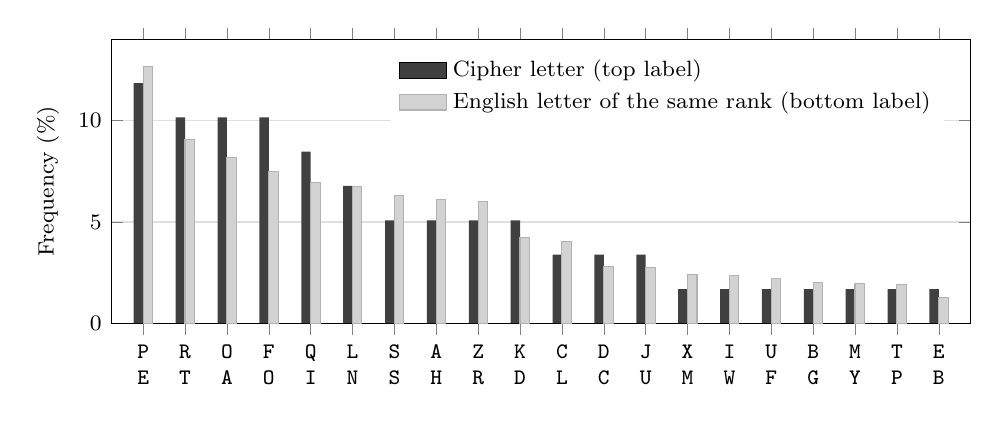
\begin{tikzpicture}
				      \begin{axis}[
						      ybar=0pt,
						      scale only axis,
						      width=0.9\linewidth,
						      height=3.6cm,
						      bar width=3.4pt,
						      ymin=0, ymax=14,
						      ylabel={Frequency (\%)},
						      ylabel style={font=\footnotesize},
						      yticklabel style={font=\footnotesize},
						      xtick=data,
						      xticklabels={{P\\E},{R\\T},{O\\A},{F\\O},{Q\\I},{L\\N},{S\\S},{A\\H},{Z\\R},{K\\D},{C\\L},{D\\C},{J\\U},{X\\M},{I\\W},{U\\F},{B\\G},{M\\Y},{T\\P},{E\\B}},
						      xticklabel style={align=center, font=\ttfamily\footnotesize},
						      enlarge x limits=0.04,
						      ymajorgrids,
						      grid style={gray!25},
						      area legend,
						      legend style={font=\footnotesize, draw=none},
						      legend cell align=left,
						      legend pos=north east,
					      ]
					      \addplot[fill=black!75, draw=none] coordinates {
							      (1,11.86) (2,10.17) (3,10.17) (4,10.17) (5,8.47) (6,6.78) (7,5.08) (8,5.08) (9,5.08) (10,5.08)
							      (11,3.39) (12,3.39) (13,3.39) (14,1.69) (15,1.69) (16,1.69) (17,1.69) (18,1.69) (19,1.69) (20,1.69)
						      };
					      \addplot[fill=gray!35, draw=gray!60] coordinates {
							      (1,12.70) (2,9.06) (3,8.17) (4,7.51) (5,6.97) (6,6.75) (7,6.33) (8,6.09) (9,5.99) (10,4.25)
							      (11,4.03) (12,2.78) (13,2.76) (14,2.41) (15,2.36) (16,2.23) (17,2.02) (18,1.97) (19,1.93) (20,1.29)
						      };
					      \legend{Cipher letter (top label), English letter of the same rank (bottom label)}
				      \end{axis}
			      \end{tikzpicture}
		      \end{center}

		      \textbf{Letter frequency alone is not enough here.}
		      The message is very short: several letters share the same count, and the ranking can easily differ from typical English.
		      (After cracking, \texttt{P} turns out to be \texttt{S}, not \texttt{E}.)
		      So letter frequency is used only as a hint, e.g.\ ``\texttt{R} and \texttt{Q} are frequent, so they may be \texttt{E}/\texttt{T},'' and the guesses are confirmed with the word analysis in (b).
	      \end{solution}
	      \myspace[v][3][mm]

	\item Knowing that this is English, what are commonly used three-letter words and two-letter words.
	      Does the knowledge give you a hint on cracking the given text?
	      \myspace[v][3][mm]
	      \begin{solution}
		      \textbf{Common English words.}
		      \begin{itemize}
			      \item \textbf{Three-letter:} \texttt{THE}, \texttt{AND}, \texttt{FOR}, \texttt{ARE}, \texttt{BUT}, \texttt{NOT}, \texttt{YOU}, \texttt{ALL}, \texttt{ANY}, \texttt{CAN},
			            \texttt{HAD}, \texttt{HER}, \texttt{WAS}, \texttt{ONE}, \texttt{OUR}, \texttt{OUT}, \texttt{HAS}, \texttt{HIS}, \texttt{HOW}, \texttt{WHO}.
			            \texttt{THE} is by far the most common word in English.
			      \item \textbf{Two-letter:} \texttt{OF}, \texttt{TO}, \texttt{IN}, \texttt{IT}, \texttt{IS}, \texttt{BE}, \texttt{AS}, \texttt{AT}, \texttt{SO}, \texttt{WE}, \texttt{HE}, \texttt{BY},
			            \texttt{OR}, \texttt{ON}, \texttt{DO}, \texttt{IF}, \texttt{ME}, \texttt{MY}, \texttt{UP}, \texttt{AN}, \texttt{GO}, \texttt{NO}, \texttt{US}, \texttt{AM}.
		      \end{itemize}

		      \textbf{Word frequency of the cipher text.}
		      The word breaks and punctuation are kept in the cipher text, so the words can be counted as well.
		      The \emph{pattern} marks which positions repeat a letter.
		      A monoalphabetic substitution never changes this pattern
		      (e.g.\ \texttt{PROVERB} and \texttt{MOLTROE} both have the pattern \texttt{ABCDEBF}).
		      \begin{center}
			      \footnotesize
			      \begin{tabular}{>{\ttfamily}lcc>{\ttfamily}l@{\hspace{2.5em}}>{\ttfamily}lcc>{\ttfamily}l}
				      \toprule
				      \normalfont Cipher word & Length & Count & \normalfont Pattern & \normalfont Cipher word & Length & Count & \normalfont Pattern \\
				      \midrule
				      FP                      & 2      & 2     & AB                  & CZSPR                   & 5      & 1     & ABCDE               \\
				      LA                      & 2      & 1     & AB                  & MOLTROE                 & 7      & 1     & ABCDEBF             \\
				      ZK                      & 2      & 1     & AB                  & PRCSOFQX                & 8      & 1     & ABCDEFGH            \\
				      QDR                     & 3      & 1     & ABC                 & LIUBROJZK               & 9      & 1     & ABCDEFGHI           \\
				      QDFP                    & 4      & 1     & ABCD                & JFPALOQSKR              & 10     & 1     & ABCDEFGHIJ          \\
				      AFOPQ                   & 5      & 1     & ABCDE               &                         &        &       &                     \\
				      \bottomrule
			      \end{tabular}
		      \end{center}

		      \textbf{Yes, it gives strong hints.}
		      Without them we would have to search all $26! \approx 4.03 \times 10^{26}$ substitution keys.
		      The word statistics cut this down to a handful of guesses:
		      \begin{itemize}
			      \item \texttt{QDR} is the \emph{only} three-letter word, so it is most likely \texttt{THE}.
			            This agrees with the letter counts from (a): \texttt{R} (6 times) and \texttt{Q} (5 times) are among the most frequent cipher letters,
			            and \texttt{E} and \texttt{T} are the two most frequent English letters.
			      \item \texttt{QDFP} starts with the same two letters as \texttt{QDR}, so it has the form \texttt{TH\_\_}
			            (\texttt{THIS}, \texttt{THAT}, \texttt{THEY}, \texttt{THEM}, \texttt{THUS}, \ldots).
			      \item \texttt{FP} is the only \emph{repeated} word, and its last letter \texttt{P} is also the last letter of \texttt{QDFP}.
			            A very common two-letter word that fits \texttt{TH\_\_} is \texttt{IS}, giving \texttt{THIS IS}.
			      \item The other two-letter words \texttt{LA} and \texttt{ZK} can only be a few common words (\texttt{OF}, \texttt{AN}, \ldots),
			            and \texttt{MOLTROE} has a repeated letter at positions 2 and 6.
			            Both facts rule out most candidates once a few letters are known.
		      \end{itemize}
		      After \texttt{T}, \texttt{H}, \texttt{E}, \texttt{I}, \texttt{S} are fixed, every longer word is already partly readable.
		      From there, the rest of the key follows word by word, as shown in (c).
	      \end{solution}
	      \myspace[v][3][mm]

	\item Cracking the given text. Measure the time that you have taken to crack this message.
	      \myspace[v][3][mm]
	      \begin{solution}
		      \textbf{Decrypted result.}
		      \begin{center}
			      \texttt{\textbf{SECURITY IS THE FIRST CAUSE OF MISFORTUNE. THIS IS AN OLD GERMAN PROVERB.}}
		      \end{center}

		      \textbf{Strategy.} Combine the letter frequencies from (a) with the word analysis from (b).
		      Guess one word at a time, starting with the words that have the fewest possible meanings.
		      Every guess fixes some cipher letters, and those letters are substituted everywhere else, which makes the next word easier.
		      To check each guess, the notebook's \texttt{candidates()} function lists all words in an English dictionary
		      (ENABLE, 172{,}823 words) that have the same letter pattern \emph{and} agree with the letters already solved.
		      \begin{center}
			      \footnotesize
			      \begin{tabularx}{\linewidth}{c>{\ttfamily}l>{\ttfamily}lXc}
				      \toprule
				      Step & \normalfont Cipher word & \normalfont Guess & Reason                                                                                                                               & \#Candidates \\
				      \midrule
				      1    & QDR                     & THE               & The only 3-letter word; \texttt{R}, \texttt{Q} are frequent (\texttt{E}, \texttt{T})                                                 & 871          \\
				      2    & FP                      & IS                & The repeated 2-letter word; also the ending of \texttt{QDFP} = \texttt{TH\_\_}                                                       & 59           \\
				      3    & QDFP                    & THIS              & \texttt{TH\_\_} with four distinct letters, ending in \texttt{S}                                                                     & 1            \\
				      4    & PRCSOFQX                & SECURITY          & \texttt{SE\_\_\_IT\_}; \texttt{SEDULITY} and \texttt{SENORITA} also match, but only \texttt{SECURITY} fits the sentence              & 3            \\
				      5    & AFOPQ                   & FIRST             & \texttt{\_IRST}                                                                                                                      & 1            \\
				      6    & CZSPR                   & CAUSE             & \texttt{C\_USE}                                                                                                                      & 1            \\
				      7    & LA                      & OF                & \texttt{\_F}                                                                                                                         & 1            \\
				      8    & JFPALOQSKR              & MISFORTUNE        & \texttt{\_ISFORTU\_E}                                                                                                                & 1            \\
				      9    & ZK                      & AN                & \texttt{A\_}, with \texttt{N} already known from step 8                                                                              & 1            \\
				      10   & MOLTROE                 & PROVERB           & \texttt{\_RO\_ER\_} with the repeated \texttt{R}                                                                                     & 1            \\
				      11   & LIUBROJZK               & OLD GERMAN        & \texttt{O\_\_\_ERMAN}; not one dictionary word (two words written without a space), solved from context ``\ldots AN \_\_\_ PROVERB'' & 0            \\
				      \bottomrule
			      \end{tabularx}
		      \end{center}
		      The partial plaintext after each step (\texttt{\_} = letter not solved yet):
		      \begin{codingbox*}[numbers=none, xleftmargin=0pt, belowskip=6pt, basicstyle=\ttfamily\footnotesize\color{editortext}]
 1  _E____T_ __ THE ____T ____E __ ______T__E. TH__ __ __ ____E____ ____E__.
 2  SE___IT_ IS THE _I_ST ___SE __ _IS___T__E. THIS IS __ ____E____ ____E__.
 3  SE___IT_ IS THE _I_ST ___SE __ _IS___T__E. THIS IS __ ____E____ ____E__.
 4  SECURITY IS THE _IRST C_USE __ _IS__RTU_E. THIS IS __ ____ER___ _R__ER_.
 5  SECURITY IS THE FIRST C_USE _F _ISF_RTU_E. THIS IS __ ____ER___ _R__ER_.
 6  SECURITY IS THE FIRST CAUSE _F _ISF_RTU_E. THIS IS A_ ____ER_A_ _R__ER_.
 7  SECURITY IS THE FIRST CAUSE OF _ISFORTU_E. THIS IS A_ O___ER_A_ _RO_ER_.
 8  SECURITY IS THE FIRST CAUSE OF MISFORTUNE. THIS IS AN O___ERMAN _RO_ER_.
 9  SECURITY IS THE FIRST CAUSE OF MISFORTUNE. THIS IS AN O___ERMAN _RO_ER_.
10  SECURITY IS THE FIRST CAUSE OF MISFORTUNE. THIS IS AN O___ERMAN PROVERB.
11  SECURITY IS THE FIRST CAUSE OF MISFORTUNE. THIS IS AN OLDGERMAN PROVERB.
\end{codingbox*}

		      \textbf{Recovered key.}
		      Writing the solved letters in plaintext-alphabet order shows the structure of the key.
		      The cipher alphabet begins with \texttt{ZECUR} and then lists the remaining letters \emph{in alphabetical order}.
		      This means the text was encrypted with a \textbf{keyword substitution cipher} using the keyword \texttt{ZECURE}
		      (``SECURE'' with \texttt{S} replaced by \texttt{Z}).
		      That structure also fills in the six letters that never appear in the message (shown in gray).
		      \begin{center}
			      \small
			      \setlength{\tabcolsep}{2.4pt}
			      \begin{tabular}{l*{26}{>{\ttfamily}c}}
				      \toprule
				      Plain  & A & B & C & D & E & F & G & H & I & \color{gray}J & \color{gray}K & L & M & N & O & P & \color{gray}Q & R & S & T & U & V & \color{gray}W & \color{gray}X & Y & \color{gray}Z \\
				      Cipher & Z & E & C & U & R & A & B & D & F & \color{gray}G & \color{gray}H & I & J & K & L & M & \color{gray}N & O & P & Q & S & T & \color{gray}V & \color{gray}W & X & \color{gray}Y \\
				      \bottomrule
			      \end{tabular}
		      \end{center}

		      \textbf{Time taken.}
		      \begin{itemize}
			      \item \textbf{By hand} (stopwatch, from first reading the cipher text to the full plaintext): \textbf{\ManualCrackTime}.
			            The first three guesses are the hardest part (871 and 59 dictionary candidates).
			            From step 3 on, every word has at most 3 candidates, so the rest is quick.
			      \item \textbf{Dictionary-assisted} (replaying the 11 guesses with \texttt{candidates()} in the notebook): \textbf{0.908 seconds}.
		      \end{itemize}
		      This shows why a substitution cipher is weak.
		      It hides the letters but keeps the letter frequencies, word lengths, and repetition patterns of the language.
		      A longer cipher text would make these statistics even clearer and the text even easier to crack.
	      \end{solution}
	      \myspace[v][3][mm]

	      \newpage

	\item Create a simple python program for cracking the Caesar cipher text using brute force attack.
	      Explain the design and demonstrate your software.
	      (You may use an English dictionary for validating results.)
	      \myspace[v][3][mm]
	      \begin{solution}
		      \textbf{Design.}
		      A Caesar cipher shifts every letter by the same secret amount $k$:
		      \[ E_k(x) = (x + k) \bmod 26, \qquad D_k(y) = (y - k) \bmod 26, \qquad k \in \{0, 1, \ldots, 25\}. \]
		      There are only 26 keys, so trying all of them is instant.
		      The only hard part is recognizing which of the 26 outputs is the real message.
		      The program (Task (d) in \texttt{code/activity-03-code.ipynb}) has four parts:
		      \begin{enumerate}[label=\arabic*.]
			      \item \textbf{Explicit key.} The secret shift is stored in the variable \texttt{KEY = 7}. \newline
			            \texttt{caesar\_encrypt(text, key)} shifts each letter forward and leaves spaces and punctuation unchanged.
			            \texttt{caesar\_decrypt} is the same function with \texttt{-key}.
			      \item \textbf{Brute force.} \texttt{brute\_force\_caesar(ciphertext)} decrypts the cipher text with \emph{every} key $0, \ldots, 25$.
			      \item \textbf{Validation with an English dictionary.} \texttt{dictionary\_score} is the fraction of letters that belong to words found in the ENABLE dictionary
			            (weighting by letters stops short words that match by chance from inflating the score).
			            Ties are broken with \texttt{chi\_squared}, the $\chi^2$ distance between the candidate's letter counts $O_c$ and the counts $E_c$ expected from English frequencies:
			            \[ \chi^2 = \sum_{c \in \{A, \ldots, Z\}} \frac{(O_c - E_c)^2}{E_c}. \]
			      \item \textbf{Decision.} The candidates are ranked by score.
			            The best one is accepted only if its dictionary score is at least \texttt{threshold = 0.8}.
			            Otherwise the program returns \texttt{None}, meaning the text is not a Caesar cipher.
		      \end{enumerate}

		      \textbf{Program.}
		      \begin{codingbox*}[language=Python, belowskip=6pt]
import re
import time
import string
import statistics
from collections import Counter

import pandas as pd

ALPHABET = string.ascii_uppercase
KEY = 7  # secret shift of the Caesar cipher
MESSAGE = "SECURITY IS THE FIRST CAUSE OF MISFORTUNE. THIS IS AN OLD GERMAN PROVERB."

# English dictionary (ENABLE word list) used to validate candidates
with open("enable1.txt", "r") as f:
    ENGLISH_WORDS = {w.strip().upper() for w in f if w.strip()}

# Relative frequency (%) of each letter in typical English text
ENGLISH_FREQ = {
    "E": 12.70, "T": 9.06, "A": 8.17, "O": 7.51, "I": 6.97, "N": 6.75, "S": 6.33,
    "H": 6.09, "R": 5.99, "D": 4.25, "L": 4.03, "C": 2.78, "U": 2.76, "M": 2.41,
    "W": 2.36, "F": 2.23, "G": 2.02, "Y": 1.97, "P": 1.93, "B": 1.29, "V": 0.98,
    "K": 0.77, "J": 0.15, "X": 0.15, "Q": 0.10, "Z": 0.07,
}

def caesar_encrypt(text, key):
    """Shift every letter `key` positions forward in the alphabet; other characters are kept."""
    return "".join(ALPHABET[(ALPHABET.index(c) + key) % 26] if c in ALPHABET else c for c in text.upper())

def caesar_decrypt(text, key):
    return caesar_encrypt(text, -key)

def dictionary_score(text):
    """Fraction of letters that belong to valid English words (1.0 = every word is in the dictionary)."""
    words = re.findall(r"[A-Z]+", text.upper())
    total = sum(len(w) for w in words)
    return sum(len(w) for w in words if w in ENGLISH_WORDS) / total if total else 0.0

def chi_squared(text):
    """Chi-squared distance from English letter frequencies (lower = more English-like)."""
    counts = Counter(c for c in text.upper() if c in ALPHABET)
    n = sum(counts.values())
    return sum((counts[c] - n * ENGLISH_FREQ[c] / 100) ** 2 / (n * ENGLISH_FREQ[c] / 100) for c in ALPHABET)

def brute_force_caesar(ciphertext, threshold=0.8):
    """Try all 26 keys; return the ranking and (key, plaintext) of the best candidate, or None."""
    rows = []
    for key in range(26):
        candidate = caesar_decrypt(ciphertext, key)
        rows.append((key, dictionary_score(candidate), chi_squared(candidate), candidate))

    ranking = pd.DataFrame(rows, columns=["key", "dictionary score", "chi-squared", "candidate plaintext"])
    ranking = ranking.sort_values(["dictionary score", "chi-squared"], ascending=[False, True], ignore_index=True)

    best = ranking.iloc[0]
    answer = (int(best["key"]), best["candidate plaintext"]) if best["dictionary score"] >= threshold else None
    return ranking, answer

# Demonstration 1: encrypt with KEY, then crack it without knowing KEY
caesar_cipher_text = caesar_encrypt(MESSAGE, KEY)
ranking, answer = brute_force_caesar(caesar_cipher_text)
recovered_key, recovered_text = answer
assert recovered_key == KEY and recovered_text == MESSAGE

# Demonstration 2: the same attack on the cipher text of this problem
ranking_given, answer_given = brute_force_caesar(
    "PRCSOFQX FP QDR AFOPQ CZSPR LA JFPALOQSKR. QDFP FP ZK LIUBROJZK MOLTROE."
)
\end{codingbox*}

		      \textbf{Demonstration 1: cracking a Caesar cipher text.}
		      The message is encrypted with \texttt{KEY = 7}, and the program then recovers it from the cipher text alone:
		      \begin{codingbox*}[numbers=none, xleftmargin=0pt, belowskip=6pt, basicstyle=\ttfamily\footnotesize\color{editortext}]
Key            : 7
Message        : SECURITY IS THE FIRST CAUSE OF MISFORTUNE. THIS IS AN OLD GERMAN PROVERB.
Cipher text    : ZLJBYPAF PZ AOL MPYZA JHBZL VM TPZMVYABUL. AOPZ PZ HU VSK NLYTHU WYVCLYI.
Recovered key  : 7
Recovered text : SECURITY IS THE FIRST CAUSE OF MISFORTUNE. THIS IS AN OLD GERMAN PROVERB.
\end{codingbox*}
		      The first rows of the ranking (full 26-row table in the notebook):
		      \begin{center}
			      \footnotesize
			      \begin{tabular}{cccl}
				      \toprule
				      Key        & Dictionary score & $\chi^2$        & Candidate plaintext (first sentence)                         \\
				      \midrule
				      \textbf{7} & \textbf{1.000}   & \textbf{15.347} & \texttt{\textbf{SECURITY IS THE FIRST CAUSE OF MISFORTUNE.}} \\
				      14         & 0.102            & 573.317         & \texttt{LXVNKBMR BL MAX YBKLM VTNLX HY FBLYHKMNGX.}          \\
				      1          & 0.068            & 1126.028        & \texttt{YKIAXOZE OY ZNK LOXYZ IGAYK UL SOYLUXZATK.}          \\
				      20         & 0.034            & 228.747         & \texttt{FRPHEVGL VF GUR SVEFG PNHFR BS ZVFSBEGHAR.}          \\
				      $\vdots$   & $\vdots$         & $\vdots$        & $\vdots$                                                     \\
				      25         & 0.000            & 1567.501        & \texttt{AMKCZQBG QA BPM NQZAB KICAM WN UQANWZBCVM.}          \\
				      \bottomrule
			      \end{tabular}
		      \end{center}
		      The correct key is clearly separated from the others: score 1.000 versus at most 0.102 for every wrong key.
		      It also has by far the lowest $\chi^2$.
		      Over 100 repeated runs, the full 26-key attack takes
		      \textbf{1.820\,ms on average} (stdev 0.680\,ms, min 1.318\,ms, max 5.916\,ms).
		      As an extra check, the program recovers the correct key for all 26 possible values of \texttt{KEY}.

		      \textbf{Demonstration 2: the given cipher text.}
		      Running the same attack on this problem's cipher text returns \texttt{None}:
		      \begin{center}
			      \footnotesize
			      \begin{tabular}{cccl}
				      \toprule
				      Key & Dictionary score & $\chi^2$ & Candidate plaintext (first sentence)                \\
				      \midrule
				      23  & 0.102            & 53.397   & \texttt{SUFVRITA IS TGU DIRST FCVSU OD MISDORTVNU.} \\
				      17  & 0.102            & 1149.848 & \texttt{YALBXOZG OY ZMA JOXYZ LIBYA UJ SOYJUXZBTA.} \\
				      25  & 0.085            & 907.408  & \texttt{QSDTPGRY GQ RES BGPQR DATQS MB KGQBMPRTLS.} \\
				      \bottomrule
			      \end{tabular}
		      \end{center}
		      No shift gives English (best score 0.102 $<$ 0.8), so the given text is \emph{not} a Caesar cipher.
		      This agrees with (c), where it turned out to be a keyword substitution cipher.
		      The two key spaces explain why brute force works for one cipher but not the other.
		      At the measured speed of about $1.820 / 26 \approx 0.07$\,ms per key:
		      \begin{itemize}
			      \item \textbf{Caesar:} 26 keys, searched in about 1.8\,ms.
			      \item \textbf{General substitution:} $26! \approx 4.03 \times 10^{26}$ keys, which would take about $8.95 \times 10^{14}$ years.
		      \end{itemize}
		      That is why the substitution cipher in (c) had to be broken with frequency and word analysis instead of trying every key.
	      \end{solution}

\end{subproblems_alpha}
\end{problem}
% ================================================================================ %

% ================================================================================ %
%                                    Problem 02                                    %
% ================================================================================ %
\begin{problem}
\textbf{(Cryptanalysis on Symmetric Encryption)}
\par Vigenère is a complex version of the Caesar cipher.
It is a polyalphabetic substitution.
\begin{subproblems_alpha}
	\item Please review \href{https://en.wikipedia.org/wiki/Kasiski_examination}{\textbf{Kasiski examination}}.
	      Explain how it can be used to attack Vigenère.
	      \myspace[v][3][mm]
	      \begin{solution}
		      \textbf{Setting.}
		      The Vigenère cipher shifts the $i$-th plaintext letter by the key letter at the same position,
		      and the key of length $m$ is repeated over the whole message:
		      \[ C_i = (P_i + K_{i \bmod m}) \bmod 26, \qquad P_i = (C_i - K_{i \bmod m}) \bmod 26. \]
		      Because the shift depends on the position, the same plaintext letter becomes different cipher letters
		      (below, \texttt{A}$\to$\texttt{C}/\texttt{P} and \texttt{T}$\to$\texttt{K}/\texttt{R}).
		      This is why the letter-frequency attack from Problem 1 does not work directly.
		      \begin{center}
			      \footnotesize
			      \setlength{\tabcolsep}{3pt}
			      \begin{tabular}{l*{12}{>{\ttfamily}c}}
				      \toprule
				      Plain  & A & T & T & A & C & K & A & T & D & A & W & N \\
				      Key    & C & R & Y & P & T & O & C & R & Y & P & T & O \\
				      \midrule
				      Cipher & C & K & R & P & V & Y & C & K & B & P & P & B \\
				      \bottomrule
			      \end{tabular}
		      \end{center}

		      \textbf{Demonstration setup.}
		      The notebook (Problem 2 in \texttt{code/activity-03-code.ipynb}) encrypts an 852-letter English paragraph with the key variable
		      \texttt{VIGENERE\_KEY = "CRYPTO"}.
		      It then attacks the cipher text \emph{without} using the key.
		      The \emph{index of coincidence}, $\mathrm{IC} = \sum_{c} f_c (f_c - 1) / \big(N(N-1)\big)$, is the probability that two letters picked at random are equal.
		      It shows how the encryption flattens the letter statistics:
		      \begin{center}
			      \footnotesize
			      \begin{tabular}{lcl}
				      \toprule
				      Text                      & IC     & Most frequent letters                                  \\
				      \midrule
				      English (expected)        & 0.0655 & --                                                     \\
				      Random letters (expected) & 0.0385 & --                                                     \\
				      Plain text                & 0.0784 & \texttt{E} 18.7\%, \texttt{T} 11.2\%, \texttt{A} 6.7\% \\
				      Vigenère cipher text      & 0.0463 & \texttt{G} 8.5\%, \texttt{C} 7.7\%, \texttt{V} 7.2\%   \\
				      \bottomrule
			      \end{tabular}
		      \end{center}
		      The cipher text looks almost random (IC close to 0.0385), and its most frequent letter is far less dominant than \texttt{E} in the plain text.

		      % -------------------------------------------------------------------------------- %
		      \par\medskip\noindent\textbf{\large 1. Purpose of the Kasiski examination}
		      % -------------------------------------------------------------------------------- %

		      The weakness of Vigenère is that the key \emph{repeats}.
		      The purpose of the Kasiski examination (published by Friedrich Kasiski in 1863) is to find the \textbf{key length $m$} from the cipher text alone.
		      Knowing $m$ is the turning point of the attack:
		      \begin{itemize}
			      \item All letters at positions $i \equiv j \pmod m$ are shifted by the same key letter.
			            The polyalphabetic cipher therefore splits into $m$ separate Caesar ciphers, and each one can be broken with the frequency analysis from Problem 1.
			      \item Instead of searching $26^m$ keys ($26^6 \approx 3.09 \times 10^8$ for \texttt{CRYPTO}),
			            the attacker only needs 26 trials per column, i.e.\ $26m = 156$ trials in total.
		      \end{itemize}

		      \textbf{Why repeated fragments reveal $m$.}
		      Suppose the same plaintext fragment appears at positions $i$ and $j$, and $j - i$ is a multiple of $m$.
		      Then both copies are encrypted with the same sequence of key letters, so the \emph{cipher text repeats as well}.
		      If the copies start at different key positions, they are encrypted differently and do not repeat.
		      So the distance between two identical cipher fragments is (very likely) a multiple of the key length.

		      \textbf{Procedure.}
		      \begin{enumerate}[label=\arabic*.]
			      \item Find sequences of at least 3 letters that occur more than once in the cipher text, and record their positions.
			      \item Compute the distance between consecutive occurrences of each sequence.
			      \item Factor every distance and count how often each factor appears.
			      \item The key length is a factor shared by (almost) all distances. Usually it is the largest such factor, but the result is only a \emph{candidate} and must be confirmed.
		      \end{enumerate}

		      \textbf{Worked example.}
		      The cipher text contains 57 repeated sequences, 15 of which have at least 4 letters.
		      The plaintext column is shown only to explain the result; the attack never sees it.
		      \begin{center}
			      \footnotesize
			      \setlength{\tabcolsep}{4pt}
			      \begin{tabular}{r>{\ttfamily}l>{\ttfamily\color{gray}}llll}
				      \toprule
				      \# & \normalfont Cipher sequence & \normalfont Plaintext (hidden) & Positions     & Distance(s) & Factorization                                \\
				      \midrule
				      1  & KFTVWRYCGMSZK               & THECIPHERTEXT                  & 463, 589      & 126         & $2 \cdot 3^2 \cdot 7$                        \\
				      2  & VYCHTAGG                    & THESAMEP                       & 156, 444      & 288         & $2^5 \cdot 3^2$                              \\
				      3  & TGEAST                      & CIPHER                         & 133, 211, 385 & 78, 174     & $2 \cdot 3 \cdot 13$,\; $2 \cdot 3 \cdot 29$ \\
				      4  & JTMHGI                      & LETTER                         & 242, 284      & 42          & $2 \cdot 3 \cdot 7$                          \\
				      5  & MUMVG                       & OFTHE                          & 290, 542      & 252         & $2^2 \cdot 3^2 \cdot 7$                      \\
				      6  & QXSP                        & BEEN                           & 21, 183       & 162         & $2 \cdot 3^4$                                \\
				      7  & TKPG                        & ERBE                           & 147, 759      & 612         & $2^2 \cdot 3^2 \cdot 17$                     \\
				      8  & GUGC                        & EDIN                           & 192, 786      & 594         & $2 \cdot 3^3 \cdot 11$                       \\
				      9  & NGGU                        & USED                           & 298, 784      & 486         & $2 \cdot 3^5$                                \\
				      10 & VYYI                        & THAT                           & 372, 738      & 366         & $2 \cdot 3 \cdot 61$                         \\
				      11 & ICEX                        & REPE                           & 409, 817      & 408         & $2^3 \cdot 3 \cdot 17$                       \\
				      12 & IASO                        & THEM                           & 423, 711      & 288         & $2^5 \cdot 3^2$                              \\
				      13 & PKFT                        & NTHE                           & 504, 588      & 84          & $2^2 \cdot 3 \cdot 7$                        \\
				      14 & PIAS                        & RTHE                           & 698, 710      & 12          & $2^2 \cdot 3$                                \\
				      15 & CKXF                        & EVER                           & 776, 812      & 36          & $2^2 \cdot 3^2$                              \\
				      \bottomrule
			      \end{tabular}
		      \end{center}
		      Every one of these distances contains the factor $2 \cdot 3 = 6$, and their GCD is 6.
		      Each repeat really is the same plaintext (e.g.\ \texttt{THECIPHERTEXT}, or \texttt{CIPHER} three times) at the same offset in the key.
		      Counting the factors of the distances gives:
		      \begin{center}
			      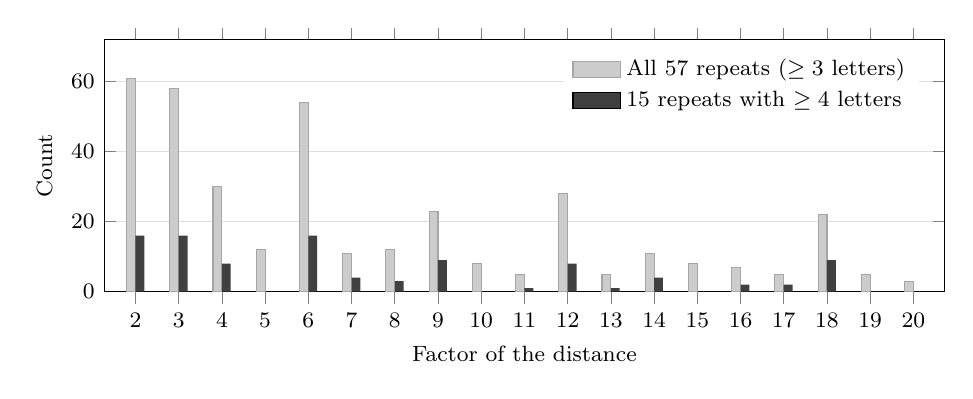
\begin{tikzpicture}
				      \begin{axis}[
						      ybar=0pt,
						      scale only axis,
						      width=0.88\linewidth,
						      height=3.2cm,
						      bar width=3.2pt,
						      ymin=0, ymax=72,
						      xlabel={Factor of the distance},
						      ylabel={Count},
						      xlabel style={font=\footnotesize},
						      ylabel style={font=\footnotesize},
						      ticklabel style={font=\footnotesize},
						      xtick={2,...,20},
						      enlarge x limits=0.04,
						      ymajorgrids,
						      grid style={gray!25},
						      area legend,
						      legend style={font=\footnotesize, draw=none},
						      legend cell align=left,
						      legend pos=north east,
					      ]
					      \addplot[fill=gray!40, draw=gray!70] coordinates {
							      (2,61) (3,58) (4,30) (5,12) (6,54) (7,11) (8,12) (9,23) (10,8) (11,5)
							      (12,28) (13,5) (14,11) (15,8) (16,7) (17,5) (18,22) (19,5) (20,3)
						      };
					      \addplot[fill=black!75, draw=none] coordinates {
							      (2,16) (3,16) (4,8) (5,0) (6,16) (7,4) (8,3) (9,9) (10,0) (11,1)
							      (12,8) (13,1) (14,4) (15,0) (16,2) (17,2) (18,9) (19,0) (20,0)
						      };
					      \legend{All 57 repeats ($\geq 3$ letters), 15 repeats with $\geq 4$ letters}
				      \end{axis}
			      \end{tikzpicture}
		      \end{center}

		      \textbf{Limitations visible in the example.}
		      \begin{itemize}
			      \item \textbf{Accidental repeats.} 19 of the 42 three-letter repeats are coincidences:
			            different plaintexts that happen to encrypt to the same letters.
			            For example, \texttt{JRQ} comes from \texttt{HAS} at position 12 and \texttt{STB} at position 31 (distance 19).
			            With all repeats included, the GCD of the distances drops to 1, and factor 2 (61) and factor 3 (58) are counted more often than 6 (54).
			            Longer repeats are much more reliable.
			      \item \textbf{Divisors of the key length.} Every multiple of 6 is also a multiple of 2 and 3.
			            So even among the clean 4-letter repeats, factors 2, 3 and 6 tie at 16.
			            Kasiski narrows the key length to the candidates $\{2, 3, 6\}$ (with 6 the most likely),
			            and it needs enough cipher text to produce aligned repeats at all.
		      \end{itemize}
		      Both problems are resolved with \textbf{superimposition}.

		      % -------------------------------------------------------------------------------- %
		      \par\medskip\noindent\textbf{\large 2. Superimposition}
		      % -------------------------------------------------------------------------------- %

		      \emph{Superimposition} means writing the cipher text on top of (a shifted copy of) itself,
		      so that letters encrypted with the \emph{same key letter} line up.
		      It serves two purposes in the attack: confirming the key length, and splitting the text into columns that can be solved one by one.

		      \textbf{(i) Superimposition test: confirming the key length.}
		      Place the cipher text over a copy of itself shifted by $s$ letters, and count the positions where the two letters are equal:
		      \begin{itemize}
			      \item If $s$ is a \textbf{multiple of $m$}, both letters were shifted by the same key letter.
			            They are equal exactly when their plaintext letters are equal, which happens with the English probability
			            $\sum_c p_c^2 \approx 0.0655$.
			      \item If $s$ is \textbf{not a multiple of $m$}, the two shifts differ and a match is pure chance: $1/26 \approx 0.0385$.
		      \end{itemize}
		      The first 36 letters, superimposed with a shift of 6, already show this.
		      At every position where the cipher letters match (\texttt{\textasciicircum}), the hidden plaintext letters also match
		      (\texttt{R}/\texttt{R}, \texttt{P}/\texttt{P}, \texttt{S}/\texttt{S}, \texttt{T}/\texttt{T}):
		      \begin{codingbox*}[numbers=none, xleftmargin=0pt, belowskip=6pt, basicstyle=\ttfamily\footnotesize\color{editortext}]
Cipher text      : EIWEMCIIYEAMJRQPEKCPQQXSPRADGHGJRQXH
Shifted by s = 6 : IIYEAMJRQPEKCPQQXSPRADGHGJRQXHYVCCMV
Coincidence      :  ^ ^          ^              ^
\end{codingbox*}
		      Over the whole cipher text, the coincidence rate for each shift $s = 1, \ldots, 24$ is:
		      \begin{center}
			      \begin{tikzpicture}
				      \begin{axis}[
						      scale only axis,
						      width=0.88\linewidth,
						      height=3.2cm,
						      bar width=5pt,
						      xmin=0.3, xmax=24.7,
						      ymin=0, ymax=9.5,
						      xlabel={Shift $s$},
						      ylabel={Coincidence rate (\%)},
						      xlabel style={font=\footnotesize},
						      ylabel style={font=\footnotesize},
						      ticklabel style={font=\footnotesize},
						      xtick={1,...,24},
						      ymajorgrids,
						      grid style={gray!25},
						      legend style={font=\footnotesize, draw=none, at={(0.5,1.03)}, anchor=south},
						      legend columns=4,
						      legend cell align=left,
					      ]
					      \addplot[ybar, bar shift=0pt, area legend, fill=gray!40, draw=gray!70] coordinates {
							      (1,4.70) (2,4.47) (3,4.00) (4,3.30) (5,5.19) (7,3.55) (8,4.62) (9,5.10) (10,3.56) (11,3.33)
							      (13,4.41) (14,3.58) (15,5.14) (16,4.31) (17,4.19) (19,3.84) (20,3.61) (21,2.65) (22,3.98) (23,4.83)
						      };
					      \addplot[ybar, bar shift=0pt, area legend, fill=black!75, draw=none] coordinates {
							      (6,6.74) (12,8.33) (18,8.03) (24,7.73)
						      };
					      \addplot[keywordcolor, thick, dashed, domain=0.3:24.7, samples=2] {6.55};
					      \addplot[black!60, thick, dotted, domain=0.3:24.7, samples=2] {3.85};
					      \legend{Other shifts, Multiples of 6, English (6.55\%), Random (3.85\%)}
				      \end{axis}
			      \end{tikzpicture}
		      \end{center}
		      Only the shifts 6, 12, 18 and 24 reach the English level (6.74--8.33\%).
		      All other shifts, including 2 (4.47\%) and 3 (4.00\%), stay near the random level.
		      The GCD of the peaks is $\gcd(6, 12, 18, 24) = 6$, which rules out the Kasiski candidates 2 and 3.

		      The same idea can be applied to columns.
		      Write the text in rows of a candidate length $m$, and average the IC of the $m$ columns:
		      \begin{center}
			      \footnotesize
			      \setlength{\tabcolsep}{2.5pt}
			      \begin{tabular}{l*{12}{c}}
				      \toprule
				      Candidate length $m$ & 1     & 2     & 3     & 4     & 5     & \textbf{6}     & 7     & 8     & 9     & 10    & 11    & 12    \\
				      Avg.\ column IC      & 0.046 & 0.051 & 0.060 & 0.051 & 0.046 & \textbf{0.078} & 0.046 & 0.051 & 0.060 & 0.051 & 0.044 & 0.080 \\
				      \bottomrule
			      \end{tabular}
		      \end{center}
		      $m = 6$ is the smallest length whose columns look like English.
		      $m = 3$ only reaches 0.060, because each of its columns mixes two key letters (\texttt{C}/\texttt{P}, \texttt{R}/\texttt{T}, \texttt{Y}/\texttt{O}).
		      $m = 12$ is also high, but only because it is a multiple of 6.
		      The program therefore takes the smallest $m$ whose average column IC is within 90\% of the best, which gives $m = 6$.

		      \textbf{(ii) Superimposition by columns: recovering the key.}
		      This is how Kasiski finished the attack.
		      Write the cipher text in rows of $m = 6$ letters, which is the same as superimposing copies of the text shifted by $6, 12, 18, \ldots$.
		      Every column now contains only letters that were shifted by \emph{one} key letter $k_j$,
		      so each of the 6 columns is an ordinary Caesar cipher with 142 letters:
		      \begin{center}
			      \footnotesize
			      \begin{tabular}{c|>{\ttfamily}c>{\ttfamily}c>{\ttfamily}c>{\ttfamily}c>{\ttfamily}c>{\ttfamily}c}
				      Row      & \normalfont$k_1$ & \normalfont$k_2$ & \normalfont$k_3$ & \normalfont$k_4$ & \normalfont$k_5$ & \normalfont$k_6$ \\
				      \hline
				      1        & E                & I                & W                & E                & M                & C                \\
				      2        & I                & I                & Y                & E                & A                & M                \\
				      3        & J                & R                & Q                & P                & E                & K                \\
				      4        & C                & P                & Q                & Q                & X                & S                \\
				      5        & P                & R                & A                & D                & G                & H                \\
				      6        & G                & J                & R                & Q                & X                & H                \\
				      $\vdots$ & $\vdots$         & $\vdots$         & $\vdots$         & $\vdots$         & $\vdots$         & $\vdots$         \\
				      142      & Q                & K                & F                & D                & E                & R                \\
			      \end{tabular}
		      \end{center}
		      Each column is then solved like the Caesar cipher in Problem 1(d).
		      A quick guess is that the column's most common letter stands for \texttt{E}.
		      A more reliable test decrypts the column with all 26 shifts and keeps the one whose letter frequencies are closest to English (lowest $\chi^2$):
		      \begin{center}
			      \footnotesize
			      \setlength{\tabcolsep}{3.5pt}
			      \begin{tabular}{cccccccc}
				      \toprule
				      Column & Letters & Most common & Key (most common $=$ \texttt{E}) & Key ($\chi^2$) & Best $\chi^2$ & 2nd-best $\chi^2$ \\
				      \midrule
				      1      & 142     & \texttt{G}  & \texttt{C}                       & \texttt{C}     & 48.99         & 369.10            \\
				      2      & 142     & \texttt{V}  & \texttt{R}                       & \texttt{R}     & 46.09         & 380.07            \\
				      3      & 142     & \texttt{C}  & \texttt{Y}                       & \texttt{Y}     & 44.34         & 462.03            \\
				      4      & 142     & \texttt{T}  & \texttt{P}                       & \texttt{P}     & 37.81         & 314.22            \\
				      5      & 142     & \texttt{X}  & \texttt{T}                       & \texttt{T}     & 14.49         & 386.01            \\
				      6      & 142     & \texttt{S}  & \texttt{O}                       & \texttt{O}     & 14.35         & 481.29            \\
				      \bottomrule
			      \end{tabular}
		      \end{center}
		      In every column, the best shift has a $\chi^2$ that is 7--33 times smaller than the second best, so each key letter is unambiguous.
		      The recovered key is \textbf{\texttt{CRYPTO}}.
		      Decrypting with it gives back the original text exactly
		      (\texttt{CRYPTOGRAPHYHASALWAYSBEENACONTESTBETWEEN\ldots}).
		      The complete attack (key length, then all 6 columns) takes \textbf{9.15\,ms on average} (stdev 1.11\,ms, 20 runs).

		      % -------------------------------------------------------------------------------- %
		      \par\medskip\noindent\textbf{\large 3. When does the attack work?}
		      % -------------------------------------------------------------------------------- %

		      Running the same attack on only the first $n$ letters of the cipher text:
		      \begin{center}
			      \footnotesize
			      \begin{tabular}{ccccc}
				      \toprule
				      Letters $n$ & Letters per column & Key length found & Recovered key                             & Correct key letters \\
				      \midrule
				      60          & 10                 & 6                & \texttt{CR\textcolor{keywordcolor}{CL}TO} & 4/6                 \\
				      120         & 20                 & 6                & \texttt{CRYPTO}                           & 6/6                 \\
				      240         & 40                 & 6                & \texttt{CRYPTO}                           & 6/6                 \\
				      480         & 80                 & 6                & \texttt{CRYPTO}                           & 6/6                 \\
				      852         & 142                & 6                & \texttt{CRYPTO}                           & 6/6                 \\
				      \bottomrule
			      \end{tabular}
		      \end{center}
		      \begin{itemize}
			      \item \textbf{Enough letters per column.}
			            The period already shows up in 60 letters.
			            But with only 10 letters per column, the frequency analysis picks the wrong shift for 2 columns.
			            From about 20 letters per column onward, the key is recovered exactly.
			            The attack needs roughly $20m$ letters, so a longer key needs proportionally more cipher text.
			      \item \textbf{No period, no attack.}
			            Both Kasiski and superimposition depend entirely on the key repeating.
			            A key that is random, as long as the message, and never reused (a one-time pad) creates no aligned repeats and no coincidence peaks,
			            so neither method finds anything.
			      \item \textbf{Lesson.} Repetition leaks structure.
			            A repeated key lets identical plaintext produce identical cipher text, which is the same weakness that ECB mode has in Problem 3.
		      \end{itemize}

		      \textbf{Program} (Problem 2 in the notebook; \texttt{chi\_squared} and \texttt{caesar\_decrypt} are reused from Problem 1(d)):
		      \begin{codingbox*}[language=Python]
from collections import defaultdict

VIGENERE_KEY = "CRYPTO"  # secret key of the Vigenere cipher


def only_letters(text):
    return "".join(c for c in text.upper() if c in ALPHABET)


def vigenere_encrypt(text, key):
    """C_i = (P_i + K_(i mod m)) mod 26 over the letters of `text`."""
    letters = only_letters(text)
    return "".join(ALPHABET[(ALPHABET.index(c) + ALPHABET.index(key[i % len(key)])) % 26] for i, c in enumerate(letters))


def vigenere_decrypt(text, key):
    """P_i = (C_i - K_(i mod m)) mod 26."""
    return "".join(ALPHABET[(ALPHABET.index(c) - ALPHABET.index(key[i % len(key)])) % 26] for i, c in enumerate(text))


# ---- Step 1: Kasiski examination ------------------------------------------------
def repeated_sequences(ciphertext, min_len=3, max_len=20):
    """Maximal repeated substrings (at least `min_len` letters) and the positions where they occur."""
    seen = defaultdict(list)
    for length in range(min_len, max_len + 1):
        for i in range(len(ciphertext) - length + 1):
            seen[ciphertext[i:i + length]].append(i)
    repeats = {s: pos for s, pos in seen.items() if len(pos) > 1}

    def extends(s, pos):
        # s is only part of a longer repeat that occurs at exactly the same places
        return any(len(repeats.get(s + c, ())) == len(pos) or len(repeats.get(c + s, ())) == len(pos) for c in ALPHABET)

    return {s: pos for s, pos in repeats.items() if not extends(s, pos)}


def factors(n, limit=20):
    return [f for f in range(2, limit + 1) if n % f == 0]


# ---- Step 2: superimposition ----------------------------------------------------
def index_of_coincidence(text):
    """Probability that two letters picked at random from `text` are the same."""
    counts = Counter(text)
    n = len(text)
    return sum(f * (f - 1) for f in counts.values()) / (n * (n - 1))


def coincidence_rate(ciphertext, shift):
    """Superimpose the cipher text on itself shifted by `shift`; percentage of aligned letters that are equal."""
    pairs = list(zip(ciphertext, ciphertext[shift:]))
    return 100 * sum(a == b for a, b in pairs) / len(pairs)


def average_column_ic(ciphertext, length):
    """Mean IC of the columns obtained by writing the cipher text in rows of `length` letters."""
    return statistics.mean(index_of_coincidence(ciphertext[i::length]) for i in range(length))


def guess_key_length(ciphertext, max_len=12, ratio=0.9):
    """Smallest length whose columns look (almost) as English as the best length; multiples of the key score alike."""
    scores = {m: average_column_ic(ciphertext, m) for m in range(1, max_len + 1)}
    best = max(scores.values())
    return min(m for m, score in scores.items() if score >= ratio * best)


# ---- Step 3: every column is a Caesar cipher ------------------------------------
def solve_column(column):
    """(chi-squared, shift) of all 26 Caesar shifts of one column, best first."""
    return sorted((chi_squared(caesar_decrypt(column, s)), s) for s in range(26))


def kasiski_attack(ciphertext):
    """Find the key length by superimposition, then solve every column as a Caesar cipher."""
    length = guess_key_length(ciphertext)
    key = "".join(ALPHABET[solve_column(ciphertext[i::length])[0][1]] for i in range(length))
    return key, vigenere_decrypt(ciphertext, key)


VIGENERE_CIPHER_TEXT = vigenere_encrypt(PLAIN_TEXT_2, VIGENERE_KEY)
recovered_key, recovered_plain = kasiski_attack(VIGENERE_CIPHER_TEXT)
assert recovered_key == VIGENERE_KEY and recovered_plain == only_letters(PLAIN_TEXT_2)
\end{codingbox*}
	      \end{solution}
\end{subproblems_alpha}
\end{problem}
% ================================================================================ %

% ================================================================================ %
%                                    Problem 03                                    %
% ================================================================================ %
\begin{problem}
\textbf{(Mode in Block Cipher)}
\par Block Cipher is designed to have more randomness in a block.
However, an individual block still utilizes the same key.
Thus, it is recommended to use a cipher mode with an initial vector, chaining or feedback between blocks.
This exercise will show you the weakness of Electronic Code Book mode
which does not include any initial vector, chaining or feedback.
\begin{subproblems_alpha}
	\item Find a bitmap image that is larger than 2000x2000 pixels.
	      Note that you may resize any image.
	      To simplify the pattern, we will change it to bitmap (1-bit per pixel) using the portable bitmap format (pbm).
	      In this example, we will use \texttt{ImageMagick} for the conversion.
	      \begin{codingbox}[language=bash, deletekeywords={in}]
$ magick convert image.jpg -resize 2000x2000 org.pbm
$
\end{codingbox}
	      \myspace[v][3][mm]
	      \begin{solution}
		      We drew our own test image with \texttt{ImageMagick}, step (a) of \texttt{code/problem3.sh}, instead of using a photo.
		      It is $2048 \times 2048$ pixels, which is larger than $2000 \times 2000$.
		      This size is deliberate: a PBM row of 2048 pixels is $2048 / 8 = 256$ bytes, which is exactly 16 AES blocks of 16 bytes.
		      So every AES block covers the same 128 pixels in every row.
		      The picture contains two kinds of content:
		      \begin{itemize}
			      \item \textbf{Large flat areas}: the title \texttt{CEDT 2110413}, a padlock, and the word \texttt{AES}. Here many 16-byte blocks are identical.
			      \item \textbf{A photo-like texture} on the left, made of dithered fractal noise. Here almost every block is different.
		      \end{itemize}
		      The conversion to a 1-bit PBM follows the handout.
		      This machine has \texttt{ImageMagick} 6, where the command is \texttt{convert} (it is \texttt{magick convert} in version 7).
		      The option \texttt{-threshold 50\%} makes every pixel pure black or white:
		      \begin{codingbox*}[language=bash, numbers=none, xleftmargin=0pt, belowskip=6pt]
$ convert image.png -resize 2048x2048 -threshold 50% org.pbm
$ identify org.pbm
org.pbm PBM 2048x2048 2048x2048+0+0 1-bit Bilevel Gray 524301B
\end{codingbox*}
		      \begin{center}
			      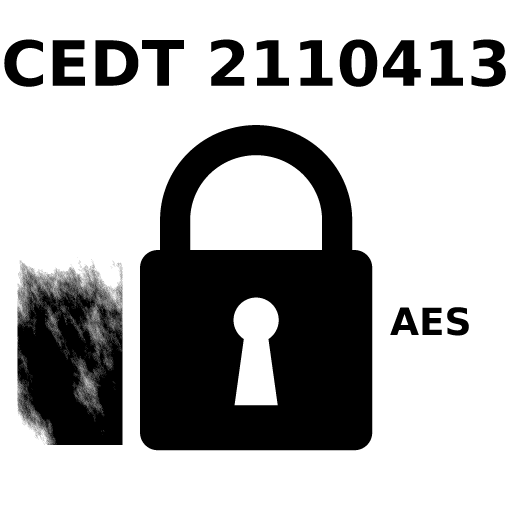
\includegraphics[width=0.35\linewidth]{images/p3-org.png}
			      \par\small Original image \texttt{org.pbm} ($2048 \times 2048$ pixels, 1 bit per pixel)
		      \end{center}
	      \end{solution}
	      \myspace[v][3][mm]
	\item The \href{https://en.wikipedia.org/wiki/Netpbm}{NetPBM} format is a naive image format
	      The first two lines contain a header (format and size in pixel).
	      Depending on the format, the pixels can be represented in either binary and ascii.
	      For our exercise, we prefer binary.
	      However, we first have to take out the header to prevent the encryption from encoding the header.
	      To do so, use your text editor (eg. vi, notepad) to take out the first two lines.
	      \begin{codingbox}[language=bash, deletekeywords={in}]
$ cp org.pbm org.x
$ vi org.x
\end{codingbox}
	      \par\texttt{P4}
	      \par\texttt{\sout{2000 2000}}
	      \par\texttt{\sout{KR)B@HD��@H�}}
	      \myspace[v][3][mm]
	      \begin{solution}
		      A binary PBM (\texttt{P4}) file is a short text header followed by the raw pixels.
		      Each pixel is 1 bit (1 = black, 0 = white), and every row is padded to a whole number of bytes:
		      \begin{center}
			      \footnotesize
			      \begin{tabular}{lll}
				      \toprule
				      Part   & Content                                    & Size                                    \\
				      \midrule
				      Line 1 & \texttt{P4} (magic number: binary bitmap)  & 3 bytes                                 \\
				      Line 2 & \texttt{2048 2048} (width and height)      & 10 bytes                                \\
				      Pixels & $2048 \times 2048$ bits, 256 bytes per row & 524{,}288 bytes $=$ 32{,}768 AES blocks \\
				      \bottomrule
			      \end{tabular}
		      \end{center}
		      The header must be removed before encryption.
		      Otherwise it would be encrypted too, and no image viewer could open the result.
		      So only the pixel data is encrypted, and the plain header is put back afterwards in (d).
		      We cut the header off with \texttt{head}/\texttt{tail} instead of \texttt{vi}, because a text editor can silently change binary data
		      (for example, by adding a newline at the end of the file):
		      \begin{codingbox*}[language=bash, numbers=none, xleftmargin=0pt, belowskip=6pt]
$ head -n 2 org.pbm > header.txt   # "P4\n2048 2048\n" = 13 bytes
$ tail -c +14 org.pbm > org.x      # pixels only: 524301 - 13 = 524288 bytes
$ xxd -c 16 -l 48 org.x            # the top rows of the image are white
$
00000000: 0000 0000 0000 0000 0000 0000 0000 0000  ................
00000010: 0000 0000 0000 0000 0000 0000 0000 0000  ................
00000020: 0000 0000 0000 0000 0000 0000 0000 0000  ................
\end{codingbox*}
		      The top of the picture is white, so \texttt{org.x} starts with thousands of identical all-zero blocks.
		      In total, only 3{,}280 of the 32{,}768 blocks are distinct, and the all-zero block alone appears 18{,}440 times (56\%).
	      \end{solution}
	      \myspace[v][3][mm]

	\item Encrypt the file with \href{https://wiki.openssl.org/index.php/Enc}{OpenSSL} with any block cipher algorithm in ECB mode (no padding and no salt).
	      \begin{codingbox}[language=bash, deletekeywords={in}]
$ openssl enc -aes-256-ecb -in org.x -nosalt -out enc.x
$
\end{codingbox}
	      \myspace[v][3][mm]
	      \begin{solution}
		      The pixel data is encrypted with AES-256 in ECB mode.
		      The key is given explicitly as a variable, a 256-bit hex value passed with \texttt{-K}, instead of being derived from a password:
		      \begin{codingbox*}[language=bash, deletekeywords={in}, numbers=none, xleftmargin=0pt, belowskip=6pt]
$ KEY=4d79af6618ab04423bd8e0e06f95f0c7156256d02e50380b1ed098d6adef1115
$ openssl enc -aes-256-ecb -e -in org.x -out enc-ecb.x -K $KEY -nopad -nosalt
$ xxd -c 16 -l 48 enc-ecb.x
00000000: 1fd8 a1dd 2b5f d9eb f4f5 76f5 47cb 3d96  ....+_....v.G.=.
00000010: 1fd8 a1dd 2b5f d9eb f4f5 76f5 47cb 3d96  ....+_....v.G.=.
00000020: 1fd8 a1dd 2b5f d9eb f4f5 76f5 47cb 3d96  ....+_....v.G.=.
\end{codingbox*}
		      \begin{itemize}
			      \item \texttt{-nopad}: the pixel data is already a whole number of blocks ($524{,}288 = 32{,}768 \times 16$), so no padding is needed.
			            Without this option, OpenSSL would add a full extra block of PKCS\#7 padding, and the file would no longer match the size in the header.
			      \item \texttt{-nosalt}: with a password (no \texttt{-K}), \texttt{openssl enc} derives the key from the password and a random salt,
			            and writes \texttt{Salted\_\_} plus the 8-byte salt in front of the cipher text.
			            Those 16 extra bytes would shift every pixel.
			            With an explicit key there is no key derivation, so no salt is written.
		      \end{itemize}
		      The cipher text is exactly as large as \texttt{org.x} (524{,}288 bytes).
		      Its first three blocks are \emph{identical}: the three white plaintext blocks were all encrypted to the same cipher block \texttt{1fd8a1dd\ldots}.
		      This is how ECB works: every block is encrypted on its own with the same key, $C_i = E_K(P_i)$.
	      \end{solution}
	      \myspace[v][3][mm]

	\item Pad the header back and see the result.
	      \begin{codingbox}[language=bash, deletekeywords={in}]
$ cp org.pbm org.x
$ vi org.x
\end{codingbox}
	      \par\texttt{\textbf{P4}}
	      \par\texttt{\textbf{2000 2000}}
	      \par\texttt{{KR)B@HD��@}}
	      \myspace[v][3][mm]
	      \begin{solution}
		      The plain header is put back in front of the cipher text (again with a shell command, not an editor), so the file is a valid PBM image again:
		      \begin{codingbox*}[language=bash, numbers=none, xleftmargin=0pt, belowskip=6pt]
$ cat header.txt enc-ecb.x > ecb.pbm
$ identify ecb.pbm
ecb.pbm PBM 2048x2048 2048x2048+0+0 1-bit Bilevel Gray 524301B
\end{codingbox*}
		      \begin{center}
			      \setlength{\tabcolsep}{6pt}
			      \begin{tabular}{cc}
				      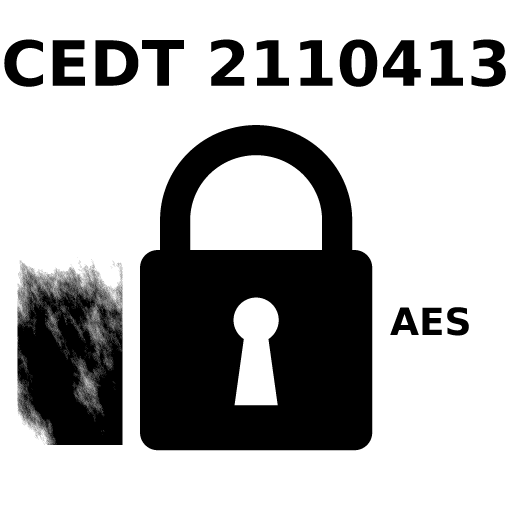
\includegraphics[width=0.35\linewidth]{images/p3-org.png} & 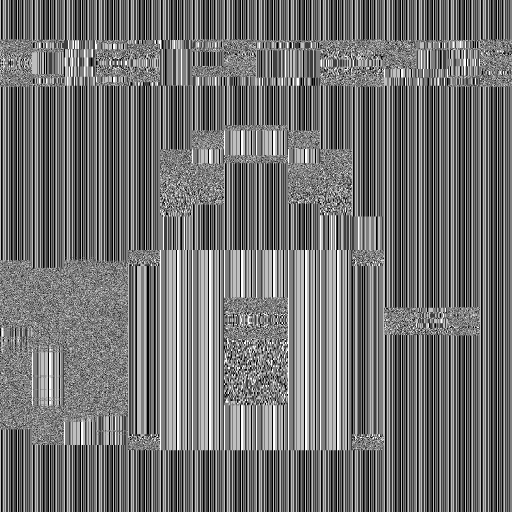
\includegraphics[width=0.35\linewidth]{images/p3-ecb.png} \\
				      \small Original                                           & \small AES-256-ECB                                        \\
			      \end{tabular}
		      \end{center}
		      \textbf{The picture is still recognizable after encryption.}
		      The title \texttt{CEDT 2110413}, the padlock with its keyhole, and the word \texttt{AES} are all clearly visible.
		      \begin{itemize}
			      \item Every \textbf{flat area} is made of identical plaintext blocks.
			            These are encrypted to identical cipher blocks, which appear as one repeated stripe pattern.
			            The white background becomes one pattern, and the black inside of the padlock becomes another.
			      \item \textbf{Edges} and the \textbf{texture} on the left contain blocks that occur only once, so they look like random noise.
			            Their \emph{outline} is still visible, though, because the flat areas around them are not random.
		      \end{itemize}
		      A zoom into $256 \times 256$ pixels around the top-left corner of the padlock (shown at $2\times$):
		      \begin{center}
			      \setlength{\tabcolsep}{4pt}
			      \begin{tabular}{ccc}
				      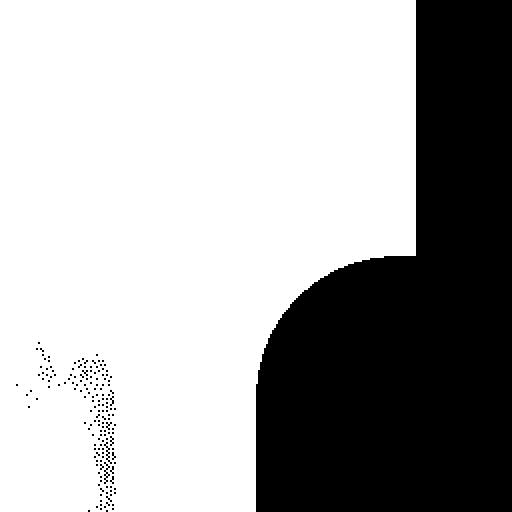
\includegraphics[width=0.25\linewidth]{images/p3-org-zoom.png} & 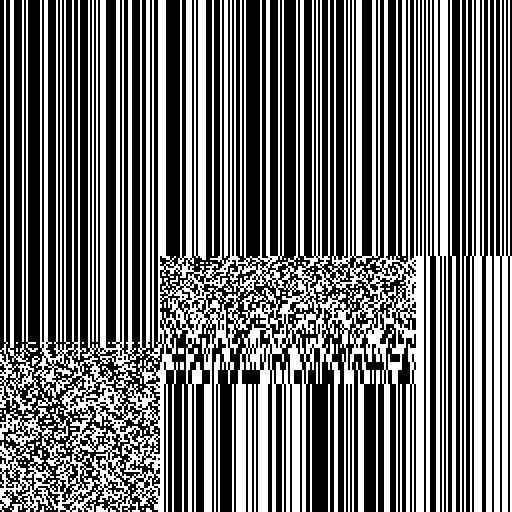
\includegraphics[width=0.25\linewidth]{images/p3-ecb-zoom.png} & 
\includegraphics[width=0.25\linewidth]{images/p3-cbc-zoom.png} \\
				      \small Original                                                & \small ECB                                                     & \small CBC (see (e))                                           \\
			      \end{tabular}
		      \end{center}
		      In the PBM file, one AES block is a strip of $16 \times 8 = 128$ pixels within a single row.
		      A row is exactly 16 blocks wide, so identical strips line up directly under each other and form vertical stripes, one pattern for each plaintext block value.
		      With a width of 2000 pixels instead, a row would be 250 bytes, which is not a multiple of 16.
		      The strips would then shift a little in every row, but the shapes would still be visible.
	      \end{solution}
	      \myspace[v][3][mm]

	\item You may try it with other modes with IV, chaining, or feedback and compare the result.
	      \myspace[v][3][mm]
	      \begin{solution}
		      The same pixel data is encrypted with the same key in four modes that use an IV together with chaining or feedback.
		      All of them use \texttt{-nopad -nosalt}, and the 128-bit IV is also given explicitly:
		      \begin{codingbox*}[language=bash, numbers=none, xleftmargin=0pt, belowskip=6pt]
$ IV=ecd0a4e1eb4570bbd396dbcccc1a0825
$ for mode in cbc cfb ofb ctr; do
      openssl enc -aes-256-$mode -e -in org.x -out enc-$mode.x -K $KEY -iv $IV -nopad -nosalt
      cat header.txt enc-$mode.x > $mode.pbm
  done
\end{codingbox*}
		      Every mode was also checked by decrypting with \texttt{-d}; each one gives back \texttt{org.x} byte for byte.
		      \begin{center}
			      \setlength{\tabcolsep}{3pt}
			      \begin{tabular}{ccc}
				      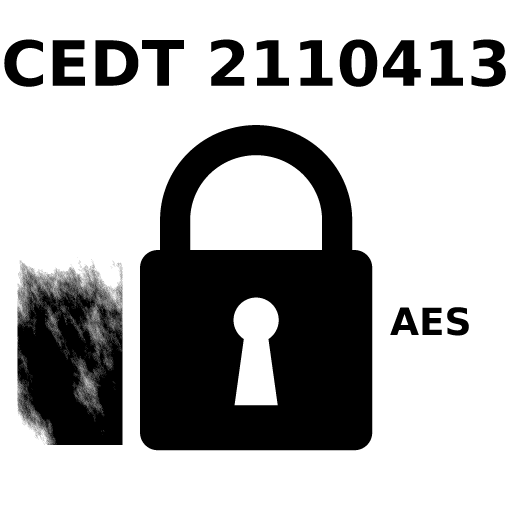
\includegraphics[width=0.3\linewidth]{images/p3-org.png} & 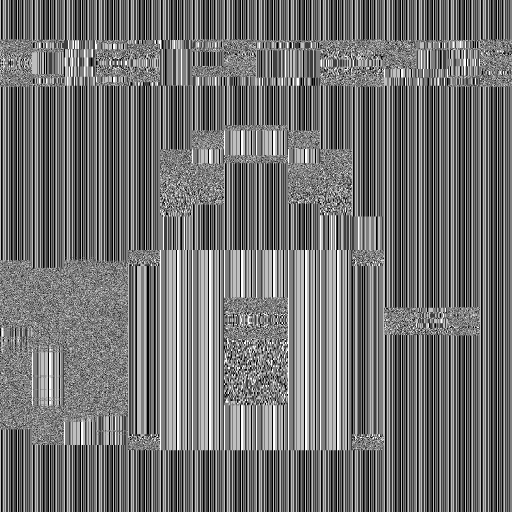
\includegraphics[width=0.3\linewidth]{images/p3-ecb.png} & 
\includegraphics[width=0.3\linewidth]{images/p3-cbc.png} \\
				      \small Original                                          & \small AES-256-ECB                                       & \small AES-256-CBC                                       \\[4pt]
				      
\includegraphics[width=0.3\linewidth]{images/p3-cfb.png} & 
\includegraphics[width=0.3\linewidth]{images/p3-ofb.png} & 
\includegraphics[width=0.3\linewidth]{images/p3-ctr.png} \\
				      \small AES-256-CFB                                       & \small AES-256-OFB                                       & \small AES-256-CTR                                       \\
			      \end{tabular}
		      \end{center}
		      CBC, CFB, OFB and CTR all give uniform noise; nothing of the picture is left.
		      Counting identical 16-byte blocks in each file puts an exact number on the difference:
		      \begin{center}
			      \footnotesize
			      \begin{tabular}{lcccc}
				      \toprule
				      File                       & Blocks   & Distinct blocks  & Most common block       & Decrypts to \texttt{org.x} \\
				      \midrule
				      \texttt{org.x} (plaintext) & 32{,}768 & 3{,}280          & 18{,}440 times          & --                         \\
				      ECB                        & 32{,}768 & \textbf{3{,}280} & \textbf{18{,}440 times} & yes                        \\
				      CBC                        & 32{,}768 & 32{,}768         & 1 time                  & yes                        \\
				      CFB                        & 32{,}768 & 32{,}768         & 1 time                  & yes                        \\
				      OFB                        & 32{,}768 & 32{,}768         & 1 time                  & yes                        \\
				      CTR                        & 32{,}768 & 32{,}768         & 1 time                  & yes                        \\
				      \bottomrule
			      \end{tabular}
		      \end{center}
		      ECB keeps \emph{exactly} the repetition structure of the plaintext: the same 3{,}280 distinct values, and the same count for the most common block.
		      Every mode with an IV and chaining or feedback turns the 32{,}768 blocks into 32{,}768 different cipher blocks.
		      The first CBC blocks show this directly.
		      They come from the same all-zero plaintext blocks as in (c), yet they are all different:
		      \begin{codingbox*}[language=bash, numbers=none, xleftmargin=0pt, belowskip=6pt, stringstyle=\color{editortext}]
$ xxd -c 16 -l 48 enc-cbc.x
$
00000000: ae1e 9f99 d677 f15d 6322 0639 6fe4 e35e  .....w.]c".9o..^
00000010: 7dbd d3ba 032d b526 00d8 cc58 fbb2 1903  }....-.&...X....
00000020: 19c6 fc61 b845 8fb5 2cc9 e3ee 0fec ff15  ...a.E..,.......
\end{codingbox*}
	      \end{solution}
	      \myspace[v][3][mm]

	\item What does the result suggest about the mode of operation in block cipher?
	      Please provide your analysis.
	      \myspace[v][3][mm]
	      \begin{solution}
		      \textbf{Why ECB leaks.}
		      In ECB every block is encrypted on its own with the same key: $C_i = E_K(P_i)$.
		      For a fixed key, $E_K$ is a fixed permutation of the $2^{128}$ possible block values.
		      Therefore $P_i = P_j \iff C_i = C_j$.
		      The cipher text hides the \emph{values} of the blocks, but it reveals exactly \emph{which blocks are equal}.
		      The experiment confirms this:
		      \begin{itemize}
			      \item The ECB file has the same 3{,}280 distinct blocks as the plaintext, and its most common block also occurs 18{,}440 times.
			            An attacker learns the whole repetition structure without breaking AES.
			      \item Any data with repeated blocks is exposed: flat image areas, long runs of zeros, file headers, fixed-format records, repeated database fields.
			            In an image, the repetition structure \emph{is} the picture.
			      \item A larger key does not help.
			            AES-256 was used, and the picture still shows, because the leak comes from the \emph{mode}, not from the cipher.
			      \item ECB is also deterministic and does not link blocks together.
			            Encrypting the same message twice gives the same cipher text.
			            An attacker can also reorder, delete or replay whole cipher blocks, and the result still decrypts without any error.
		      \end{itemize}

		      \textbf{How an IV, chaining and feedback fix it.}
		      The other modes make each block's encryption depend on the IV and on either the previous blocks or the block's position.
		      As a result, equal plaintext blocks no longer give equal cipher blocks (figure in (e)):
		      \begin{center}
			      \footnotesize
			      \renewcommand{\arraystretch}{1.3}
			      \begin{tabularx}{\linewidth}{l>{\raggedright\arraybackslash}p{4.1cm}>{\raggedright\arraybackslash}X>{\raggedright\arraybackslash}X}
				      \toprule
				      Mode & Encryption                                                        & What makes equal blocks differ              & A bit error in $C_i$ damages       \\
				      \midrule
				      ECB  & $C_i = E_K(P_i)$                                                  & nothing (deterministic)                     & all of $P_i$                       \\
				      CBC  & $C_i = E_K(P_i \oplus C_{i-1})$, $C_0 = \mathrm{IV}$              & random, unpredictable IV and chaining       & all of $P_i$, one bit of $P_{i+1}$ \\
				      CFB  & $C_i = P_i \oplus E_K(C_{i-1})$, $C_0 = \mathrm{IV}$              & IV and feedback of the cipher text          & one bit of $P_i$, all of $P_{i+1}$ \\
				      OFB  & $C_i = P_i \oplus O_i$, $O_i = E_K(O_{i-1})$, $O_0 = \mathrm{IV}$ & IV (key stream does not depend on the data) & the same bit of $P_i$ only         \\
				      CTR  & $C_i = P_i \oplus E_K(\mathrm{nonce} \,\|\, i)$                   & unique nonce and a counter                  & the same bit of $P_i$ only         \\
				      \bottomrule
			      \end{tabularx}
		      \end{center}
		      \begin{itemize}
			      \item \textbf{Padding:} ECB and CBC encrypt whole blocks, so they need padding when the data is not a multiple of 16 bytes.
			            CFB, OFB and CTR use AES to build a stream cipher and need no padding.
			      \item \textbf{Speed:} ECB and CTR can encrypt and decrypt all blocks in parallel, and CTR also allows random access.
			            CBC and CFB encryption is sequential (their decryption can run in parallel), and OFB is sequential in both directions.
		      \end{itemize}

		      \textbf{An IV only helps if it is used correctly.}
		      Two extra experiments in \texttt{code/problem3.sh} reuse the \emph{same} key and IV:
		      \begin{itemize}
			      \item \textbf{CBC with a fixed IV is deterministic again.}
			            Encrypting \texttt{org.x} twice gives byte-identical cipher texts, so an attacker can tell when the same message, or one with the same beginning, is sent twice.
			            The IV must be random and unpredictable for every message.
			      \item \textbf{CTR (and OFB) with a reused nonce produce the same key stream $S$ twice.}
			            Encrypting a second image (\texttt{TOP SECRET}) with the same key and IV gives
			            $C_1 \oplus C_2 = (P_1 \oplus S) \oplus (P_2 \oplus S) = P_1 \oplus P_2$.
			            The attacker gets the XOR of the two pictures without knowing the key:
		      \end{itemize}
		      \begin{center}
			      \setlength{\tabcolsep}{3pt}
			      \begin{tabular}{ccc}
				      
\includegraphics[width=0.3\linewidth]{images/p3-ctr.png} & 
\includegraphics[width=0.3\linewidth]{images/p3-ctr2.png} & 
\includegraphics[width=0.3\linewidth]{images/p3-ctr-xor.png} \\
				      \small $C_1$ = CTR(\texttt{org.pbm})                     & \small $C_2$ = CTR(second image)                          & \small $C_1 \oplus C_2 = P_1 \oplus P_2$                     \\
			      \end{tabular}
		      \end{center}
		      Each cipher text on its own looks random, but their XOR shows both pictures on top of each other.

		      \textbf{Conclusion.}
		      \begin{itemize}
			      \item A strong block cipher is not enough on its own: the \emph{mode of operation} decides whether patterns leak.
			            ECB should not be used for data longer than one block.
			      \item Use a mode with an IV and chaining or feedback, such as CBC with a random IV or CTR with a unique nonce.
			            Never reuse an IV or nonce with the same key.
			      \item These modes only protect confidentiality; none of them detects tampering.
			            For example, in CTR an attacker can flip chosen plaintext bits by flipping cipher text bits.
			            In practice, use an authenticated mode such as AES-GCM (CTR plus an authentication tag), which gives both confidentiality and integrity.
		      \end{itemize}
	      \end{solution}
\end{subproblems_alpha}


\par\noindent If you got it all right, the result should be like this.
\fig[0.6\linewidth]{images/ecb_example.png}{Example of ECB mode weakness}{fig:ecb_example}
\end{problem}
% ================================================================================ %

% ================================================================================ %
%                                    Problem 04                                    %
% ================================================================================ %
\begin{problem}
\textbf{(Encryption Protocol - Digital Signature)}
\begin{subproblems_alpha}
	\item Measure the performance of a hash function (sha1), RC4, Blowfish and DSA.
	      Outline your experimental design.
	      (Please use OpenSSL for your measurement)
	      \myspace[v][3][mm]
	      \begin{solution}
		      \subsection*{Experimental Design}

		      The performance of SHA-1, RC4, Blowfish, and DSA was measured using the OpenSSL \texttt{speed} command.
		      All tests should be performed on the same machine and under similar system load to ensure a fair comparison.

		      Before the experiment, the OpenSSL version and CPU information can be recorded using:

		      \begin{codingbox}[language=bash, deletekeywords={in}]
$ openssl version
$ lscpu
\end{codingbox}

		      Each test can be run for 10 seconds and repeated several times to obtain an average result.

		      \subsubsection*{SHA-1}

		      SHA-1 performance is measured as hashing throughput:

		      \begin{codingbox}[language=bash, deletekeywords={in}]
$ openssl speed -elapsed -seconds 10 sha1
$
\end{codingbox}

		      The result is reported in bytes/s or MB/s. Higher throughput means that more data can be hashed per second.

		      \subsubsection*{RC4}

		      RC4 performance is measured as encryption throughput:

		      \begin{codingbox}[language=bash, deletekeywords={in}]
$ openssl speed -elapsed -seconds 10 rc4
$
\end{codingbox}

		      For OpenSSL 3.x, the legacy provider may be required:

		      \begin{codingbox}[language=bash, deletekeywords={in}]
$ openssl speed -elapsed -seconds 10 \
$     -provider default -provider legacy rc4
\end{codingbox}

		      \subsubsection*{Blowfish}

		      Blowfish-CBC can be measured using:

		      \begin{codingbox}[language=bash, deletekeywords={in}]
openssl speed -elapsed -seconds 10 bf-cbc
\end{codingbox}

		      For OpenSSL 3.x:

		      \begin{codingbox}[language=bash, deletekeywords={in}]
$ openssl speed -elapsed -seconds 10 \
$     -provider default -provider legacy bf-cbc
\end{codingbox}

		      RC4 and Blowfish can be compared using their throughput in MB/s.

		      \subsubsection*{DSA}

		      DSA is a digital signature algorithm, so its performance should not be measured in MB/s.
		      Instead, the number of signing and verification operations per second is measured.

		      For example:

		      \begin{codingbox}[language=bash, deletekeywords={in}]
$ openssl speed -elapsed -seconds 10 dsa2048
$
\end{codingbox}

		      The important results are:

		      \begin{itemize}
			      \item signatures per second,
			      \item verifications per second.
		      \end{itemize}

		      \subsubsection*{Result Comparison}

		      The results can be summarized as follows:

		      \begin{center}
			      \begin{tabular}{|l|l|l|}
				      \hline
				      \textbf{Algorithm} & \textbf{Metric}     & \textbf{Result} \\
				      \hline
				      SHA-1              & Throughput at 16 KB & 655.42 MB/s     \\
				      RC4                & Throughput at 16 KB & 421.35 MB/s     \\
				      Blowfish           & Throughput at 16 KB & 161.82 MB/s     \\
				      DSA-2048           & Signatures/s        & 2000.5          \\
				      DSA-2048           & Verifications/s     & 2500.8          \\
				      \hline
			      \end{tabular}
		      \end{center}

		      SHA-1, RC4, and Blowfish are compared using data throughput,
		      while DSA is evaluated using the number of signature operations per second
		      because it performs a different type of cryptographic operation.

		      It should also be noted that SHA-1 and RC4 are considered obsolete
		      for modern secure applications;
		      this experiment measures their performance only.
	      \end{solution}
	      \myspace[v][3][mm]

	\item Comparing performance and security provided by each method.
	      \myspace[v][3][mm]
	      \begin{solution}
		      \subsection*{Comparison of Performance and Security}

		      The four algorithms provide different types of security services, so their performance should be compared together with their intended purpose.

		      \begin{center}
			      \begin{tabular}{|l|l|l|l|}
				      \hline
				      \textbf{Algorithm} & \textbf{Type} & \textbf{Performance} & \textbf{Security} \\
				      \hline
				      SHA-1              &
				      Hash function      &
				      Very fast          &
				      Weak / obsolete                                                               \\
				      \hline
				      RC4                &
				      Stream cipher      &
				      Very fast          &
				      Insecure                                                                      \\
				      \hline
				      Blowfish           &
				      Block cipher       &
				      Fast               &
				      Moderate, but outdated                                                        \\
				      \hline
				      DSA                &
				      Digital signature  &
				      Much slower        &
				      Strong if modern parameters are used                                          \\
				      \hline
			      \end{tabular}
		      \end{center}

		      \subsubsection*{SHA-1}

		      SHA-1 is generally fast because hashing requires only symmetric-style computations and does not involve expensive public-key operations.

		      However, SHA-1 is no longer considered secure for collision resistance. Practical collision attacks have been demonstrated, meaning that two different messages can be constructed with the same SHA-1 hash. Therefore, SHA-1 should not be used for modern digital signatures or security-sensitive applications.

		      \subsubsection*{RC4}

		      RC4 usually has very high performance because it is a simple stream cipher and requires relatively few computations per byte.

		      However, RC4 contains several statistical weaknesses in its output stream and is considered insecure for modern cryptographic applications. Therefore, although RC4 may provide good performance, its security is insufficient.

		      \subsubsection*{Blowfish}

		      Blowfish is a symmetric block cipher and generally provides good encryption throughput. It is usually slower than RC4 but still much faster than public-key algorithms such as DSA.

		      Blowfish itself has no practical attack against its full-round design when used correctly. However, it uses a relatively small 64-bit block size, which becomes problematic when encrypting large amounts of data. For this reason, newer ciphers such as AES are generally preferred.

		      \subsubsection*{DSA}

		      DSA is much slower than SHA-1, RC4, and Blowfish because it performs computationally expensive public-key operations.

		      However, DSA provides a different security service. It provides:

		      \begin{itemize}
			      \item message authentication,
			      \item message integrity, and
			      \item digital signatures.
		      \end{itemize}

		      DSA does not provide confidentiality because it is not an encryption algorithm.

		      Its security depends on the key size, hash function, and correct generation of the per-signature random value. With appropriate parameters, DSA provides significantly stronger security properties than SHA-1 or RC4, although at a higher computational cost.

		      \subsubsection*{Conclusion}

		      In general, there is a trade-off between performance and security functionality. SHA-1, RC4, and Blowfish are relatively fast because they use inexpensive operations, while DSA is slower because it uses public-key cryptography.

		      However, high performance does not necessarily mean good security. RC4 and SHA-1 are no longer considered secure, while Blowfish is outdated mainly because of its 64-bit block size. DSA can provide strong digital-signature security when appropriate parameters are used, but with significantly lower performance.

		      Therefore, the algorithms can be summarized as:

		      \[
			      \text{RC4/SHA-1/Blowfish: high throughput}
		      \]

		      \[
			      \text{DSA: lower performance but provides digital signatures}
		      \]

		      The choice of algorithm should therefore depend not only on performance, but also on the required security property.
	      \end{solution}
	      \myspace[v][3][mm]

	\item Explain the mechanism underlying Digital Signature.
	      How does it combine the strength and weakness of each encryption scheme?
	      \myspace[v][3][mm]
	      \begin{solution}
		      \subsection*{Mechanism of Digital Signature}

		      A digital signature combines a \textbf{cryptographic hash function} with \textbf{asymmetric cryptography}.
		      Its purpose is to provide message integrity, authentication, and non-repudiation.

		      The signing process can be summarized as follows:

		      \begin{enumerate}
			      \item The sender computes a hash of the message:
			            \[
				            h = H(M),
			            \]
			            where $M$ is the message and $H$ is a cryptographic hash function.

			      \item The sender uses their \textbf{private key} to generate a digital signature from the hash:
			            \[
				            S = \operatorname{Sign}_{K_{\mathrm{private}}}(h).
			            \]

			      \item The sender sends both the original message $M$ and signature $S$ to the receiver.

			      \item The receiver calculates the hash of the received message:
			            \[
				            h' = H(M).
			            \]

			      \item The receiver uses the sender's \textbf{public key} to verify the signature:
			            \[
				            \operatorname{Verify}_{K_{\mathrm{public}}}(h',S).
			            \]

			            If the verification succeeds,
			            the receiver can conclude that the message has not been modified
			            and that the signature was generated by the owner of the corresponding private key.
		      \end{enumerate}

		      For DSA specifically, the hash is not simply ``encrypted with the private key.''
		      Instead, DSA uses mathematical operations involving the private key
		      and a per-signature value to produce the signature.
		      The basic idea, however, remains that the private key is required to create the signature
		      while the public key can be used to verify it.

		      \subsubsection*{Combination of Strengths}

		      Digital signatures combine the advantages of hashing and asymmetric cryptography.

		      \begin{itemize}
			      \item \textbf{Hash functions} such as SHA-1 are very fast
			            and can reduce a message of any size into a small fixed-size digest.
			            Therefore, the expensive public-key operation does not need to process the entire message.

			      \item \textbf{Asymmetric algorithms} such as DSA allow the private key
			            to remain secret while the public key can be distributed freely.
			            This provides authentication and allows anyone with the public key to verify the signature.
		      \end{itemize}

		      Therefore, instead of applying a slow public-key operation to a large message,
		      only the much smaller hash value is signed:

		      \[
			      \text{Large Message}
			      \xrightarrow{\text{Fast Hash}}
			      \text{Small Digest}
			      \xrightarrow{\text{Public-Key Signature}}
			      \text{Digital Signature}.
		      \]

		      This gives both good efficiency and strong authentication.

		      \subsubsection*{Weaknesses}

		      The security of a digital signature depends on both components.
		      If either component is weak, the entire signature system may become insecure.

		      For example, SHA-1 has known collision attacks.
		      If an attacker can create two different messages with the same hash,

		      \[
			      H(M_1)=H(M_2),
		      \]

		      a signature associated with one message may potentially be abused
		      with another specially constructed message.
		      Therefore, modern systems use stronger hash functions such as SHA-256 instead of SHA-1.

		      DSA also depends on secure private-key management
		      and correct generation of its per-signature value.
		      If the private key or this value is exposed or generated incorrectly,
		      the signature security can be broken.

		      \subsubsection*{Relation to Symmetric Encryption}

		      Symmetric algorithms such as RC4 or Blowfish are very fast
		      and are suitable for encrypting large amounts of data,
		      but both communicating parties must share the same secret key.
		      They mainly provide \textbf{confidentiality}, not digital signatures.

		      A practical secure communication system can therefore combine both approaches:

		      \[
			      \text{Digital Signature}
			      \rightarrow
			      \text{Authentication + Integrity}
		      \]

		      \[
			      \text{Symmetric Encryption}
			      \rightarrow
			      \text{Confidentiality}.
		      \]

		      For example, a message may first be digitally signed
		      and then encrypted using a symmetric cipher.
		      This combines the high performance of symmetric encryption
		      with the authentication and integrity provided by digital signatures.

		      \subsubsection*{Conclusion}

		      Digital signatures combine the speed of cryptographic hash functions
		      with the authentication capability of asymmetric cryptography.
		      Hashing makes the process efficient,
		      while public-key cryptography allows signatures to be verified without sharing the private key.

		      However, the overall security is limited by the weakest component.
		      A weak hash function, insecure private key,
		      or incorrectly implemented signature algorithm can compromise
		      the complete digital-signature system.
		      Digital signatures also do not provide confidentiality by themselves,
		      so encryption must be used separately when confidentiality is required.
	      \end{solution}
\end{subproblems_alpha}
\end{problem}
% ================================================================================ %

\newpage

\par\noindent\textit{Hint:} \textbf{(OpenSSL command line)}
\begin{codingbox}[language=bash, deletekeywords={in}]
# List algorithms
$ openssl list cipher-algorithms
# To encrypt
$ openssl enc -ciphername [options] -e -in filename -out filename \
    -K key -iv IV -nopad -nosalt
\end{codingbox}

\end{document}
